% =====================================================================
%  Phase 2 Report -- Acrobot (single column, one-and-a-half spacing)
%  Sections I-V: Phase 1 (model); Sections VI-IX: Phase 2 (stability)
% =====================================================================
\documentclass[10pt,letterpaper]{article}
\usepackage[top=0.5in,bottom=0.55in,left=0.7in,right=0.7in]{geometry}
\usepackage[T1]{fontenc}
\usepackage{mathptmx}\usepackage{amssymb}\renewcommand{\ttdefault}{pcr}
\usepackage{amsmath,graphicx,booktabs,array,microtype,xcolor,float}
\usepackage[compact]{titlesec}
\usepackage[labelsep=period,font=footnotesize]{caption}
\usepackage{enumitem}
\usepackage{cite}
\usepackage{xurl}
\usepackage{setspace}\onehalfspacing
\usepackage[hidelinks]{hyperref}

\renewcommand{\thesection}{\Roman{section}}
\renewcommand{\thesubsection}{\Alph{subsection}}
\titleformat{\section}{\normalfont\normalsize\scshape\bfseries}{\thesection.}{0.5em}{}
\titlespacing*{\section}{0pt}{5pt plus 2pt minus 1pt}{1pt plus 1pt}
\titleformat{\subsection}[runin]{\normalfont\normalsize\itshape\bfseries}{\thesubsection.}{0.4em}{}[.]
\titlespacing*{\subsection}{0pt}{3pt plus 1pt minus 1pt}{0.6em}
\renewcommand{\thetable}{\Roman{table}}
\captionsetup[figure]{name=Fig.,skip=2pt}
\captionsetup[table]{name=Table,labelfont=bf,skip=2pt}
\setlength{\parindent}{0pt}
\setlength{\parskip}{0pt}
\setlength{\abovedisplayskip}{2pt plus 1pt minus 1pt}
\setlength{\belowdisplayskip}{2pt plus 1pt minus 1pt}
\setlength{\abovedisplayshortskip}{0pt}
\setlength{\belowdisplayshortskip}{1pt}
\setlength{\intextsep}{3pt plus 1pt minus 2pt}
\setlist{leftmargin=1.1em,itemsep=0pt,topsep=1pt,parsep=0pt}
\setlength{\emergencystretch}{1.5em}
\allowdisplaybreaks\clubpenalty=0\widowpenalty=0\displaywidowpenalty=0
\newcommand{\Nm}{\,\mathrm{N\,m}}
\hyphenpenalty=10000\exhyphenpenalty=10000
\pagestyle{plain}

\begin{document}

\begin{center}
\begin{singlespace}
{\fontsize{17}{20}\selectfont Phase 2: Stability Analysis of the Acrobot}\\[4pt]
{\small Bhargav (2025102061) \quad Sreekar (2025102074) \quad Kaushik (2025102071) \quad Divijat (2025102040)}\\[1pt]
{\footnotesize Control Systems Project \quad$\cdot$\quad Phase 2 Report (extends Phase 1) \quad$\cdot$\quad October 29, 2026}
\end{singlespace}
\end{center}
\vspace{-6pt}
{\small\textbf{Abstract.} Sections~I--V restate the Phase~1 model: the given Acrobot dynamics, its four zero-torque equilibria, their linearizations and the transfer functions from the elbow torque $\tau$ to both joint angles. Sections~VI--IX are Phase~2. We determine the stability of every equilibrium from the transfer functions and from the state matrix, and the two agree. We confirm every conclusion with a PyBullet simulation of the nonlinear model. At the upright equilibrium we show that no static or PD feedback from a single joint angle can stabilize it, because of real right-half-plane zeros. A dynamic observer-based controller can, but only for perturbations of about $1^\circ$ under the $20\Nm$ torque limit.\par}

% =====================================================================
\section{Nonlinear Model}
% =====================================================================
\noindent\begin{minipage}[t]{0.6\textwidth}\vspace{0pt}
\subsection{System and Parameters}
Two-link pendulum (Fig.~\ref{fig:schematic}) with a passive shoulder and a motor at the elbow [1], [2].
\begin{itemize}
\item Angles: $q_1$ = link~1 from the downward vertical; $q_2$ = link~2 relative to link~1; $\varphi=q_1+q_2$.
\item State: $x=[q_1,\;q_2,\;\dot q_1,\;\dot q_2]^T$.
\item Input: elbow motor torque $\tau$, $|\tau|\le20\Nm$, the only quantity we command ($\tau=0$ in this phase; set by a controller in later phases).
\item $m_1=m_2=1$~kg, $l_1=1$~m, $l_2=2$~m, $l_{c1}=0.5$~m, $l_{c2}=1$~m, $I_1=0.083$, $I_2=0.33$~kg\,m$^2$, $g=9.81$~m/s$^2$.
\end{itemize}
\subsection{Given Equations of Motion}
\begin{equation}
M(q)\ddot q+C(q,\dot q)\dot q=\tau_g(q)+B\tau,\qquad B=[0,\;1]^T\label{eq:eom}
\end{equation}
($B$ applies $\tau$ to the elbow equation only; $c_2=\cos q_2$, $s_2=\sin q_2$.)
\end{minipage}\hfill
\begin{minipage}[t]{0.36\textwidth}\vspace{0pt}
\centering
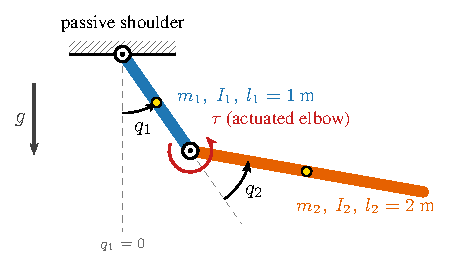
\includegraphics[width=\linewidth]{acrobot_diagram.pdf}
\captionof{figure}{Acrobot schematic (to scale); dots mark the centres of mass.}\label{fig:schematic}
\end{minipage}

\subsection{Derivation}
\textit{1) Potential energy and gravity torque:}
\begin{equation}
U=-(m_1l_{c1}+m_2l_1)g\cos q_1-m_2l_{c2}g\cos\varphi=-14.715\cos q_1-9.81\cos\varphi,\qquad
\tau_g=-\frac{\partial U}{\partial q}=-9.81\begin{bmatrix}1.5\sin q_1+\sin\varphi\\ \sin\varphi\end{bmatrix}.\label{eq:tg}
\end{equation}
\textit{2) Kinetic energy and inertia matrix:} the velocity of centre~2 is the elbow velocity ($l_1\dot q_1$) plus the rotation about the elbow ($l_{c2}\dot\varphi$), at angle $q_2$ apart (law of cosines):
\begin{equation}
T=\tfrac12(m_1l_{c1}^2+I_1)\dot q_1^2+\tfrac12I_2\dot\varphi^2+\tfrac12m_2\big(l_1^2\dot q_1^2+l_{c2}^2\dot\varphi^2+2l_1l_{c2}c_2\dot q_1\dot\varphi\big)=\tfrac12\dot q^TM\dot q,\quad
M(q)=\begin{bmatrix}2.663+2c_2 & 1.33+c_2\\ 1.33+c_2 & 1.33\end{bmatrix}.\label{eq:M}
\end{equation}
\textit{3) Coriolis term (Euler--Lagrange):} with $\partial T/\partial\dot q=M\dot q$ and $\dot M=\frac{\partial M}{\partial q_2}\dot q_2=-s_2\dot q_2\left[\begin{smallmatrix}2&1\\1&0\end{smallmatrix}\right]$,
\begin{equation}
\frac{d}{dt}\frac{\partial T}{\partial\dot q}-\frac{\partial T}{\partial q}=\tau_g+B\tau
\;\Rightarrow\; M\ddot q+\underbrace{\Big(\dot M\dot q-\frac{\partial T}{\partial q}\Big)}_{=\,C\dot q}=\tau_g+B\tau,
\qquad C(q,\dot q)=s_2\begin{bmatrix}-2\dot q_2 & -\dot q_2\\ \dot q_1 & 0\end{bmatrix}.\label{eq:C}
\end{equation}
These are the same $\tau_g$, $M$ and $C$ as in the given model.
\subsection{State-Space Form}
$M$ is always invertible, so solving~\eqref{eq:eom} for $\ddot q$ gives the state equation:
\begin{equation}
\det M=(2.663+2c_2)(1.33)-(1.33+c_2)^2=1.7729-c_2^2\ge0.7729>0\;\;(c_2^2\le1),\qquad
\dot x=f(x,\tau)=\begin{bmatrix}\dot q\\ M^{-1}\big(\tau_g+B\tau-C\dot q\big)\end{bmatrix}.\label{eq:f}
\end{equation}

% =====================================================================
\section{Equilibria}
% =====================================================================
\subsection{Conditions}
At rest $\dot q=\ddot q=0$, and the input torque is given as $\tau^*=0$. Then~\eqref{eq:eom} gives $\tau_g(q^*)=0$:
\begin{equation*}
\text{row 2: }\sin(q_1^*+q_2^*)=0,\qquad
\text{row 1: }1.5\sin q_1^*+\underbrace{\sin(q_1^*+q_2^*)}_{=0}=0\;\Rightarrow\;\sin q_1^*=0 .
\end{equation*}
\subsection{Solutions}
$q_1^*\in\{0,\pi\}$, $q_1^*+q_2^*\in\{0,\pi\}$ $\Rightarrow$ $q_2^*\in\{0,\pi\}$ (mod $2\pi$): \textbf{four equilibria}, all with both links vertical (Table~\ref{tab:eq}).

\begin{table}[h]
\centering
\caption{Equilibria for $\tau^*=0$}\label{tab:eq}
\footnotesize\setlength{\tabcolsep}{6pt}\renewcommand{\arraystretch}{0.9}
\begin{tabular}{@{}clcrl@{}}
\toprule
 & Posture & $(q_1^*,q_2^*)$ & $U$ [J] & Description\\
\midrule
$E_1$ & down--down & $(0,0)$ & $-24.525$ & both links hanging\\
$E_2$ & down--up & $(0,\pi)$ & $-4.905$ & link 1 down, link 2 up\\
$E_3$ & up--up & $(\pi,0)$ & $+24.525$ & fully upright (target)\\
$E_4$ & up--down & $(\pi,\pi)$ & $+4.905$ & link 1 up, link 2 down\\
\bottomrule
\end{tabular}
\end{table}

% =====================================================================
\section{Linearization}
% =====================================================================
\subsection{Deviation Variables}
$\tilde q=[q_1-q_1^*,\;q_2-q_2^*]^T$, $\tilde x=[\tilde q;\dot{\tilde q}]=x-x^*$, $\tilde\tau=\tau-\tau^*=\tau$. First-order Taylor expansion of~\eqref{eq:f} about $(x^*,0)$, using $f(x^*,0)=0$: $\dot{\tilde x}\approx\frac{\partial f}{\partial x}\big|_*\tilde x+\frac{\partial f}{\partial\tau}\big|_*\tilde\tau$.
\subsection{Jacobians}
\textit{Top half:} $\tfrac{d}{dt}\tilde q=\dot{\tilde q}$ $\Rightarrow$ rows $[\,0\;\;I_2\,]$. \textit{Bottom half:} $h=M^{-1}(\tau_g+B\tau-C\dot q)$; at $(x^*,0)$, $\partial(C\dot q)/\partial\dot q=0$ ($C\dot q$ is quadratic in $\dot q$, $\dot q^*=0$) and $(\partial M^{-1}/\partial q)(\tau_g+B\tau)=0$ ($\tau_g(q^*)=0$, $\tau^*=0$). Hence
\begin{equation}
\ddot{\tilde q}=P\tilde q+r\tilde\tau,\quad P=M(q^*)^{-1}K(q^*),\quad r=M(q^*)^{-1}B,\qquad
K(q^*)=\frac{\partial\tau_g}{\partial q}\Big|_{q^*}=-9.81\begin{bmatrix}1.5\cos q_1^*+\cos\varphi^* & \cos\varphi^*\\ \cos\varphi^* & \cos\varphi^*\end{bmatrix}.\label{eq:K}
\end{equation}
\subsection{Linear State-Space Model}
Stacking both halves, with the joint angles as outputs, $y=\tilde q=[q_1-q_1^*,\;q_2-q_2^*]^T$:
\begin{equation}
\boxed{\;\dot{\tilde x}=A\tilde x+B_\ell\tilde\tau,\quad y=C_y\tilde x+D\tilde\tau,\qquad
A=\begin{bmatrix}0 & I_2\\ P & 0\end{bmatrix}\!,\;
B_\ell=\begin{bmatrix}0\\ r\end{bmatrix}\!,\;
C_y=\begin{bmatrix}I_2 & 0\end{bmatrix}\!,\; D=0\;}\label{eq:AB}
\end{equation}
\subsection{Example: $E_1=(0,0)$} $\cos q_1^*=\cos\varphi^*=c_2=1$:
\begin{gather*}
K=\begin{bmatrix}-24.525&-9.81\\-9.81&-9.81\end{bmatrix}\!,\quad
M=\begin{bmatrix}4.663&2.33\\2.33&1.33\end{bmatrix}\!,\quad
\det M=0.7729,\quad M^{-1}=\frac{1}{0.7729}\begin{bmatrix}1.33&-2.33\\-2.33&4.663\end{bmatrix}\!,\\
P_{E1}=M^{-1}K=\begin{bmatrix}-12.6292&12.6926\\14.7488&-29.6119\end{bmatrix}\!,\qquad
r_{E1}=\begin{bmatrix}-3.0147\\6.0332\end{bmatrix}\!.
\end{gather*}

\noindent\begin{minipage}[t]{0.42\textwidth}\vspace{0pt}
\subsection{All Equilibria}
$M$ depends only on $q_2^*$; $K$ only on the signs of $\cos q_1^*$, $\cos\varphi^*$. Upside down, gravity flips: $K_{E3}=-K_{E1}$ with $M_{E3}=M_{E1}$, so $P_{E3}=-P_{E1}$; likewise $P_{E4}=-P_{E2}$. Results in Table~\ref{tab:lin}; with~\eqref{eq:AB} they give $(A,B_\ell,C_y,D)$ at each equilibrium.
\end{minipage}\hfill
\begin{minipage}[t]{0.55\textwidth}\vspace{2pt}
\centering
\captionof{table}{Linearization results ($\det M=0.7729$ at all four)}\label{tab:lin}
\footnotesize\setlength{\tabcolsep}{4pt}\renewcommand{\arraystretch}{1.0}
\begin{tabular}{@{}ccccc@{}}
\toprule
 & $(\cos q_1^*,\cos\varphi^*)$ & $M(q^*)$ & $P=M^{-1}K$ & $r=M^{-1}B$\\
\midrule
$E_1$ & $(1,1)$ & $\left[\begin{smallmatrix}4.663&2.33\\2.33&1.33\end{smallmatrix}\right]$ & $\left[\begin{smallmatrix}-12.6292&12.6926\\14.7488&-29.6119\end{smallmatrix}\right]$ & $\left[\begin{smallmatrix}-3.0147\\6.0332\end{smallmatrix}\right]$\\
$E_2$ & $(1,-1)$ & $\left[\begin{smallmatrix}0.663&0.33\\0.33&1.33\end{smallmatrix}\right]$ & $\left[\begin{smallmatrix}-12.6292&12.6926\\10.5095&4.2266\end{smallmatrix}\right]$ & $\left[\begin{smallmatrix}-0.4270\\0.8578\end{smallmatrix}\right]$\\
$E_3$ & $(-1,-1)$ & as $E_1$ & $-P_{E1}$ & $r_{E1}$\\
$E_4$ & $(-1,1)$ & as $E_2$ & $-P_{E2}$ & $r_{E2}$\\
\bottomrule
\end{tabular}
\end{minipage}

% =====================================================================
\section{Transfer Functions}
% =====================================================================
\subsection{Laplace Transform}
With $\tilde Q_i(s)=\mathcal L\{\tilde q_i(t)\}$, $\tilde{\mathcal T}(s)=\mathcal L\{\tilde\tau(t)\}$, $\tilde Q=[\tilde Q_1,\tilde Q_2]^T$ and zero initial conditions ($\ddot{\tilde q}\to s^2\tilde Q$):
\begin{equation*}
s^2\tilde Q=P\tilde Q+r\tilde{\mathcal T}\;\Rightarrow\;(s^2I-P)\,\tilde Q(s)=r\,\tilde{\mathcal T}(s),\qquad
(s^2I-P)^{-1}=\frac{1}{\Delta(s)}\begin{bmatrix}s^2-P_{22}&P_{12}\\P_{21}&s^2-P_{11}\end{bmatrix}\!,\quad
\Delta(s)=s^4-\operatorname{tr}(P)\,s^2+\det P .
\end{equation*}
\subsection{General Formula} Multiplying by $r$ and dividing each row by $\tilde{\mathcal T}$ ($G_i=\tilde Q_i/\tilde{\mathcal T}$):
\begin{equation}
\boxed{\;G_1(s)=\frac{r_1s^2+(P_{12}r_2-P_{22}r_1)}{\Delta(s)},\qquad
G_2(s)=\frac{r_2s^2+(P_{21}r_1-P_{11}r_2)}{\Delta(s)}\;}\label{eq:G}
\end{equation}
\textit{Poles:} roots of $\Delta$ (= eigenvalues of $A$); with $\lambda=s^2$, $\lambda^2-\operatorname{tr}(P)\lambda+\det P=0$, then $s=\pm\sqrt\lambda$.
\textit{Zeros:} $s^2=-(P_{12}r_2-P_{22}r_1)/r_1$ for $G_1$ and $s^2=-(P_{21}r_1-P_{11}r_2)/r_2$ for $G_2$.

\noindent\begin{minipage}{\linewidth}
\subsection{Example: $E_1$}
$\operatorname{tr}P=-42.2410$, $\det P=186.7719$ $\Rightarrow$ $\lambda=s^2=-5.018,\,-37.224$ $\Rightarrow$ poles $\pm j2.2400,\ \pm j6.1011$; numerator constants $P_{12}r_2-P_{22}r_1=-12.6926$, $P_{21}r_1-P_{11}r_2=31.7316$ $\Rightarrow$ $G_1=-3.0147\,(s^2+4.2103)/\Delta$, $G_2=6.0332\,(s^2+5.2595)/\Delta$ (row $E_1$ of Table~\ref{tab:tf}).
\end{minipage}

\begin{table}[h]
\centering
\caption{Transfer functions $G_i(s)=N_i(s)/\Delta(s)$ at the four equilibria}\label{tab:tf}
\footnotesize\setlength{\tabcolsep}{4pt}\renewcommand{\arraystretch}{0.85}
\begin{tabular}{@{}cllllll@{}}
\toprule
 & Denominator $\Delta(s)$ (monic) & $N_1(s)$ \;($\tau\to q_1$) & $N_2(s)$ \;($\tau\to q_2$) & Poles & Zeros of $G_1$ & Zeros of $G_2$\\
\midrule
$E_1$ & $s^4+42.2410\,s^2+186.7719$ & $-3.0147\,(s^2+4.2103)$ & $6.0332\,(s^2+5.2595)$ & $\pm j2.2400,\ \pm j6.1011$ & $\pm j2.0519$ & $\pm j2.2934$\\
$E_2$ & $s^4+8.4025\,s^2-186.7719$ & $-0.4270\,(s^2-29.7273)$ & $0.8578\,(s^2+7.3982)$ & $\pm3.1775,\ \pm j4.3010$ & $\pm5.4523$ & $\pm j2.7200$\\
$E_3$ & $s^4-42.2410\,s^2+186.7719$ & $-3.0147\,(s^2-4.2103)$ & $6.0332\,(s^2-5.2595)$ & $\pm2.2400,\ \pm6.1011$ & $\pm2.0519$ & $\pm2.2934$\\
$E_4$ & $s^4-8.4025\,s^2-186.7719$ & $-0.4270\,(s^2+29.7273)$ & $0.8578\,(s^2-7.3982)$ & $\pm4.3010,\ \pm j3.1775$ & $\pm j5.4523$ & $\pm2.7200$\\
\bottomrule
\end{tabular}
\end{table}

\subsection{All Equilibria}
Table~\ref{tab:tf}. With no friction only even powers of $s$ occur, so poles and zeros come in pairs $\pm p$; since $P_{E3}=-P_{E1}$, each $\pm j\omega$ at $E_1$ becomes $\pm\omega$ at $E_3$ (likewise $E_2$/$E_4$).

% =====================================================================
% =====================================================================
\section{Verification of the Model (Phase 1)}
% =====================================================================
\noindent\begin{minipage}[t]{0.66\textwidth}\vspace{0pt}
\begin{itemize}
\item The model derivation and all values in Tables~\ref{tab:lin} and~\ref{tab:tf} were verified in MATLAB (agreement to four decimals).
\item Nonlinear~\eqref{eq:f} vs.\ linear~\eqref{eq:AB}, from the same small deviation with $\tau=0$ (Fig.~\ref{fig:sim}): near $E_1$ from $\tilde q(0)=(0.1,-0.1)$~rad they agree within $1.0^\circ$ ($q_1$) and $2.0^\circ$ ($q_2$) over 8~s. Near $E_3$ from $\tilde q_1(0)=10^{-3}$~rad the error is $0.02\%$ when $|\tilde q_1|=1^\circ$.
\item With $\tau=0$, $T+U$ stays constant to $10^{-8}$ (no friction).
\item Phase~1 animation: \href{https://drive.google.com/file/d/18Ic6QdsY37QBfvFIwmVA_8Z-u4AyNPdg/view?usp=sharing}{\textcolor{blue!60!black}{\textbf{watch the video}}}.
\end{itemize}
\end{minipage}\hfill
\begin{minipage}[t]{0.31\textwidth}\vspace{-26pt}
\centering
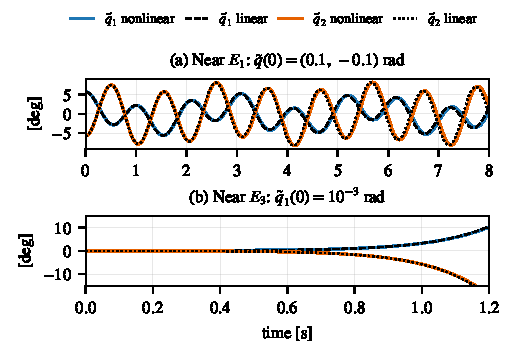
\includegraphics[width=\linewidth]{sim.pdf}
\captionof{figure}{Nonlinear (colour) vs.\ linear (black) responses near (a) $E_1$, (b) $E_3$.}\label{fig:sim}
\end{minipage}

% =====================================================================
\section{Stability: Criteria (Phase 2)}
% =====================================================================
\subsection{Two Views of the Same Poles}
\textit{State space:} the linear model~\eqref{eq:AB} is asymptotically stable iff every eigenvalue of $A$ has $\operatorname{Re}<0$. It is unstable if any eigenvalue has $\operatorname{Re}>0$. It is marginally stable (bounded, non-decaying) if the eigenvalues on the imaginary axis are simple and none lies to the right of it.
\textit{Transfer functions:} $G_1,G_2$ in~\eqref{eq:G} are BIBO stable iff every pole has $\operatorname{Re}<0$.
\textit{Nonlinear system:} by Lyapunov's indirect method, an eigenvalue with $\operatorname{Re}>0$ makes the equilibrium of~\eqref{eq:f} unstable, while eigenvalues on the imaginary axis leave the question open [5].

The two views give the same poles here. At every equilibrium $\operatorname{rank}[B_\ell\;AB_\ell\;A^2B_\ell\;A^3B_\ell]=4$ (controllable), and $(A,C_j)$ with $C_j=e_j^T$ has observability rank $4$ for $j=1$ and $j=2$. Each $G_j$ is therefore a minimal realization, with no pole--zero cancellation (in Table~\ref{tab:tf} no zero equals a pole). So the poles of $G_1$ and $G_2$ are exactly the eigenvalues of $A$, and the transfer-function verdict and the state-space verdict must coincide.

\subsection{What the Characteristic Polynomial Allows}
$\det(sI-A)=\Delta(s)=s^4-\operatorname{tr}(P)\,s^2+\det P$ has no $s^3$ and no $s^1$ term, because the model has no friction. All coefficients of a Hurwitz polynomial are positive, so \textbf{no equilibrium can be asymptotically stable with $\tau=0$}; at best it is marginally stable. With $\lambda=s^2$ (the eigenvalues of $P$),
\begin{equation}
\lambda^2-\operatorname{tr}(P)\,\lambda+\det P=0:\qquad
\lambda<0\Rightarrow s=\pm j\sqrt{-\lambda}\ \ \text{(oscillation)},\qquad
\lambda>0\Rightarrow s=\pm\sqrt{\lambda}\ \ \text{(one pole in the RHP)}.\label{eq:lam}
\end{equation}
Hence $\det P<0$ gives one $\lambda$ of each sign (one RHP pole). $\det P>0$ with $\operatorname{tr}P<0$ gives two negative $\lambda$ (all poles on the $j\omega$-axis). $\det P>0$ with $\operatorname{tr}P>0$ gives two positive $\lambda$ (two RHP poles).

\subsection{Link to the Potential Energy}
$K=\partial\tau_g/\partial q=-\nabla^2U$ (the Hessian of~\eqref{eq:tg}) and $M\succ0$. $P=M^{-1}K$ is similar to the symmetric matrix $M^{-1/2}KM^{-1/2}$, which is congruent to $K$. By Sylvester's law of inertia, $P$ has as many positive eigenvalues as $\nabla^2U$ has negative ones [3]. So \textbf{the number of RHP poles equals the number of directions in which $U$ decreases}: a minimum of $U$ gives none, a saddle one, a maximum two.

% =====================================================================
\section{Stability of Each Equilibrium}
% =====================================================================
\begin{table}[h]
\centering
\caption{Stability of the four equilibria from the transfer functions ($G_1,G_2$), the state matrix ($A$) and the energy}\label{tab:stab}
\footnotesize\setlength{\tabcolsep}{3.5pt}\renewcommand{\arraystretch}{0.95}
\begin{tabular}{@{}cccccccl@{}}
\toprule
 & $\operatorname{tr}P$, $\det P$ & $\lambda=\operatorname{eig}P$ & poles of $G_1,G_2$ $=$ eig$(A)$ & $\operatorname{eig}\nabla^2U$ & $U$ at $q^*$ & RHP & verdict (linear / nonlinear)\\
\midrule
$E_1$ & $-42.241,\ 186.772$ & $-5.018,\ -37.224$ & $\pm j2.2400,\ \pm j6.1011$ & $4.905,\ 29.43$ & minimum & 0 & marginally stable / Lyapunov stable\\
$E_2$ & $-8.403,\ -186.772$ & $-18.499,\ 10.096$ & $\pm3.1775,\ \pm j4.3010$ & $-14.715,\ 9.81$ & saddle & 1 & unstable / unstable\\
$E_3$ & $42.241,\ 186.772$ & $5.018,\ 37.224$ & $\pm2.2400,\ \pm6.1011$ & $-29.43,\ -4.905$ & maximum & 2 & unstable / unstable\\
$E_4$ & $8.403,\ -186.772$ & $-10.096,\ 18.499$ & $\pm4.3010,\ \pm j3.1775$ & $-9.81,\ 14.715$ & saddle & 1 & unstable / unstable\\
\bottomrule
\end{tabular}
\end{table}

\subsection{$E_1$ (down--down): Marginally Stable, Lyapunov Stable}
\textit{Transfer functions:} the poles $\pm j2.2400$ and $\pm j6.1011$ are simple and on the imaginary axis, so $G_1$ and $G_2$ are \emph{not} BIBO stable. A bounded input at a resonance, e.g.\ $\tau=\sin(2.24t)$, produces a response that grows like $t\sin(2.24t)$.
\textit{State space:} the same eigenvalues make the free response a bounded, undamped sum of two modes, so $E_1$ is marginally stable, not asymptotically stable.
\textit{Nonlinear:} linearization is inconclusive here, but energy settles it. Take $V(x)=\tfrac12\dot q^TM\dot q+U(q)-U(q^*)$. It is positive definite near $E_1$ because $\nabla^2U\succ0$ there (eigenvalues $4.905,\,29.43$). Along~\eqref{eq:eom}, $\dot V=\dot q^TB\tau=0$ for $\tau=0$. So $E_1$ is \textbf{stable in the sense of Lyapunov}, and not asymptotically stable: $V$ is constant, so the swing never decays.

\subsection{$E_2$ and $E_4$: Saddles, One RHP Pole Each}
$\det P=-186.772<0$, so by~\eqref{eq:lam} each has one real RHP pole ($+3.1775$ at $E_2$, $+4.3010$ at $E_4$) plus an undamped pair ($\pm j4.3010$, $\pm j3.1775$). Both $G_j$ are BIBO unstable and $A$ is unstable. By Lyapunov's indirect method both nonlinear equilibria are unstable. $U$ is a saddle at each: one link sits up, so the energy decreases along exactly one direction.

\subsection{$E_3$ (up--up): Maximum, Two RHP Poles}
Gravity flips, so $P_{E3}=-P_{E1}$ and $\lambda$ changes sign. The poles $\pm j2.24,\pm j6.10$ of $E_1$ become $\pm2.2400$ and $\pm6.1011$. With two RHP poles, $E_3$ is unstable (transfer function, state space and nonlinear). $U$ has a strict maximum, so every direction leads downhill.

% =====================================================================
\section{Simulation Evidence}
% =====================================================================
\subsection{Simulator}
All Phase~2 simulations use the full nonlinear model in \textbf{PyBullet} [6] (Featherstone multibody dynamics, uniform rods, no joint damping, step $0.25$~ms). It is checked against an RK4 integration of the given equations~\eqref{eq:eom}: with $q(0)=(0.8,-0.5)$~rad and $\tau=3\sin2t$, the joint angles agree within $0.52^\circ$ over 5~s. The same simulator runs the linear model~\eqref{eq:AB} alongside, from the same initial condition.

\begin{figure}[H]
\centering
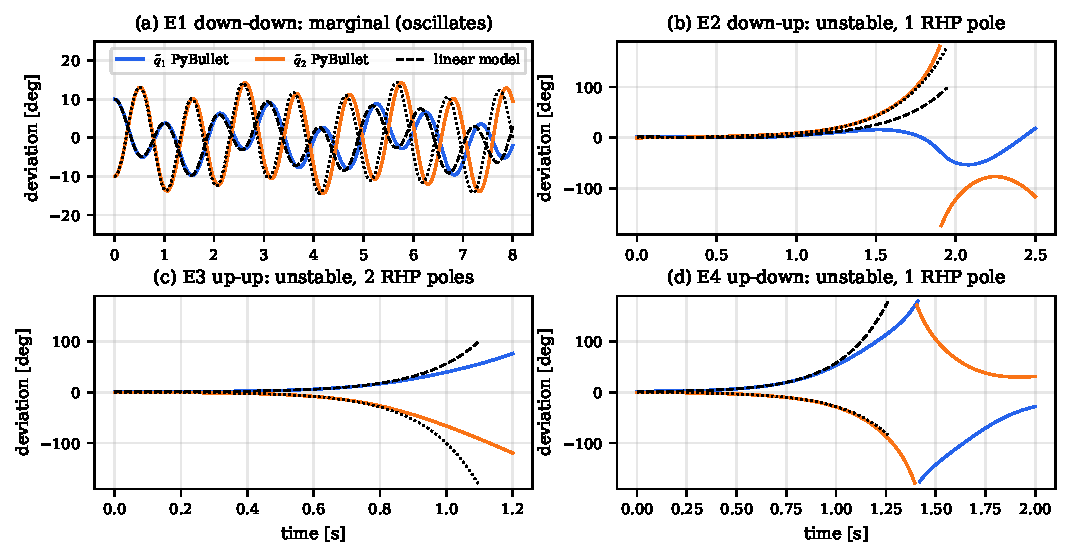
\includegraphics[width=0.92\textwidth]{fig_openloop.pdf}
\caption{Free response ($\tau=0$) near each equilibrium: PyBullet (colour) vs.\ linear model (black). Initial offsets: (a) $\tilde q(0)=(10^\circ,-10^\circ)$; (b) $2^\circ$; (c) $1^\circ$; (d) $2^\circ$ on $q_1$.}\label{fig:ol}
\end{figure}

\subsection{Each Conclusion Confirmed}
\begin{itemize}
\item \textbf{$E_1$:} the response stays bounded at its initial $10^\circ$ amplitude and never decays (Fig.~\ref{fig:ol}a), as marginal stability predicts. Over 60~s the energy changes by only $1.2\times10^{-3}$~J, which is integration error. The spectrum of $\tilde q_1$ peaks at $2.239$ and $5.997$~rad/s (Fig.~\ref{fig:growth}b). These are the poles $\pm j2.240$ and $\pm j6.101$, the second within one frequency bin ($2\pi/60=0.105$~rad/s) of a 60~s record.
\item \textbf{$E_2,E_3,E_4$:} a tiny offset grows until the arm falls (Fig.~\ref{fig:ol}b--d). The linear model tracks it until about $20^\circ$, then over-predicts. On a log scale the growth is a straight line (Fig.~\ref{fig:growth}a). Its slope is $3.171$, $6.088$ and $4.294$~s$^{-1}$, against the largest RHP poles $3.1775$, $6.1011$ and $4.3010$ (errors $0.22\%$, $0.21\%$, $0.15\%$). The time to reach $30^\circ$ is $2.52$~s from $0.05^\circ$ ($E_2$), $1.55$~s from $0.01^\circ$ ($E_3$) and $1.69$~s from $0.05^\circ$ ($E_4$).
\end{itemize}
\begin{figure}[H]
\centering
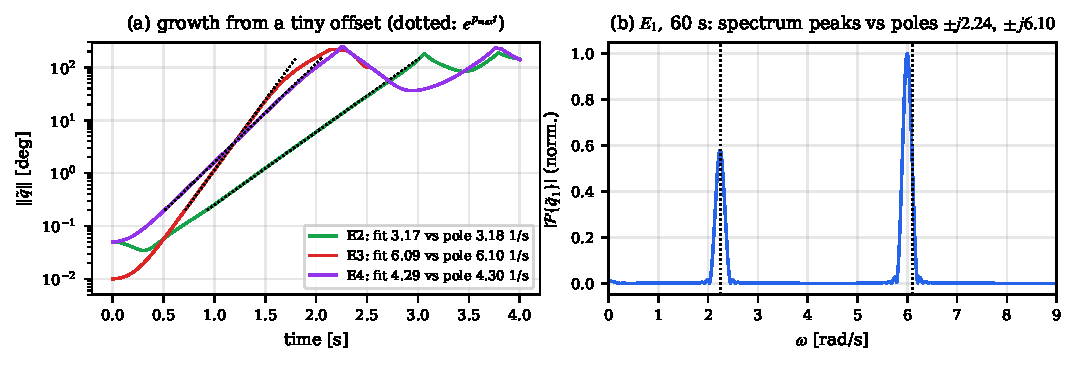
\includegraphics[width=0.92\textwidth]{fig_growth.pdf}
\caption{(a) $\|\tilde q\|$ from a tiny offset; dotted lines have slope equal to the largest RHP pole. (b) Spectrum of $\tilde q_1$ near $E_1$ over 60~s; dotted lines are the poles.}\label{fig:growth}
\end{figure}

% =====================================================================
\section{Single-Angle Feedback at the Upright Equilibrium $E_3$}
% =====================================================================
\subsection{Problem}
Only one joint angle $y=\tilde q_j$ ($j=1$ or $2$) is measured, and the elbow torque is $\tau=-C(s)\,y$. With $G_j=N_j/\Delta$ and $C=N_c/D_c$, the closed-loop poles are the roots of $\Delta D_c+N_jN_c$. At $E_3$ (Table~\ref{tab:tf}):
\begin{equation}
\Delta=s^4\underbrace{-42.241}_{a_2}s^2+\underbrace{186.772}_{a_0},\qquad
N_1=\underbrace{-3.0147}_{b_2}s^2+\underbrace{12.6926}_{b_0}\ (\text{zeros }\pm2.0519),\qquad
N_2=\underbrace{6.0332}_{b_2}s^2\underbrace{-31.7316}_{b_0}\ (\text{zeros }\pm2.2934).\label{eq:e3tf}
\end{equation}

\subsection{Static or PD Feedback Cannot Stabilize It}
With $C(s)=K_p+K_ds$ the closed-loop polynomial is
\begin{equation}
s^4+(K_db_2)\,s^3+(a_2+K_pb_2)\,s^2+(K_db_0)\,s+(a_0+K_pb_0).\label{eq:pdpoly}
\end{equation}
Hurwitz requires every coefficient to be positive, so $K_db_2>0$ \emph{and} $K_db_0>0$, i.e.\ $b_2$ and $b_0$ must have the same sign. For both angles they have opposite signs ($b_0/b_2=-z^2$), \textbf{because the zeros $\pm z$ are real: one lies in the RHP}. No $K_p$, $K_d$ can satisfy both conditions. Pure proportional feedback ($K_d=0$) is worse still: \eqref{eq:pdpoly} is even in $s$, so its roots are symmetric about the imaginary axis and can never all lie in the LHP.

Root-locus view: at low gain the closed-loop poles sit near the open-loop RHP poles $2.24$ and $6.10$. As the gain grows they move to the zeros of $(K_p+K_ds)N_j$, one of which is the RHP zero $+z$. So every gain leaves a pole in the RHP.

A grid search over $K_p\in[-400,400]$, $K_d\in[-150,150]$ (Fig.~\ref{fig:pd}a,b) confirms this. The smallest attainable largest real part is $0.96$~s$^{-1}$ for $q_1$ (at $K_p=-15$, $K_d=0$) and $2.29$ for $q_2$. The latter is approached at high gain, where a pole tends to the RHP zero $2.2934$. In PyBullet even these best gains let a $1^\circ$ offset reach $30^\circ$ in $1.0$~s ($q_1$) and $1.8$~s ($q_2$) (Fig.~\ref{fig:pd}c).
\begin{figure}[H]
\centering
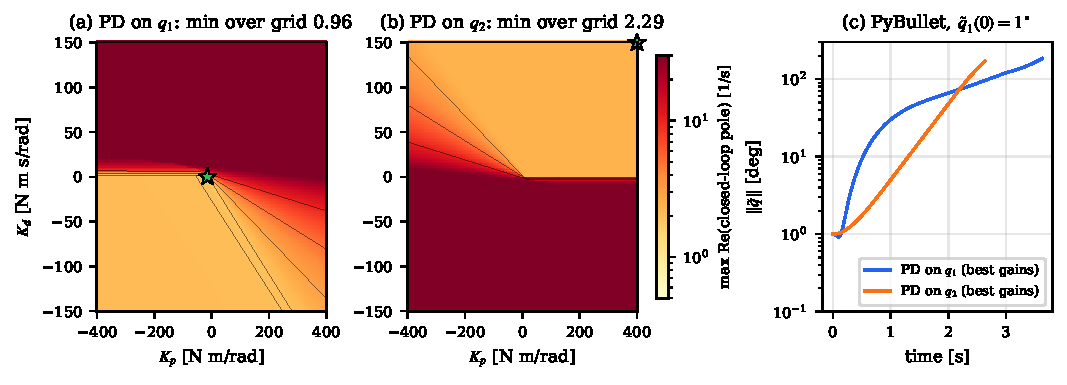
\includegraphics[width=0.95\textwidth]{fig_pd.pdf}
\caption{PD feedback from one angle at $E_3$. (a, b) Largest real part of the closed-loop poles over the gain plane; it is positive everywhere (star: best gains). (c) PyBullet with the best gains: the arm still falls.}\label{fig:pd}
\end{figure}

\subsection{A Dynamic (Observer-Based) Controller Can, in Principle}
Since $(A,C_j)$ is observable for both angles (Sec.~VI-A), a Luenberger observer $\dot{\hat x}=A\hat x+B_\ell\tau+L(y-C_j\hat x)$ reconstructs the whole state from one angle. Feedback $\tau=-K\hat x$ on the estimate then gives closed-loop poles $\operatorname{eig}(A-B_\ell K)\cup\operatorname{eig}(A-LC_j)$ (separation principle).
\begin{itemize}
\item \textit{Gains:} $K$ is from LQR with $Q=\operatorname{diag}(10,10,1,1)$, $R=1$: $K=[-266.1,\,-107.4,\,-115.0,\,-54.3]$, with $\operatorname{eig}(A-B_\ell K)=-10.09,\,-4.25,\,-2.24\pm0.04j$. $L$ is from the dual LQR problem: observer poles $-6.34,-5.88,-2.67,-1.90$ for $q_1$ and $-6.56,-5.67,-2.49,-2.03$ for $q_2$. All are in the LHP, so the linearized loop is asymptotically stable.
\item \textit{Stable controller or not (parity interlacing [4]):} a stable stabilizing controller exists iff every interval between consecutive real RHP zeros (including $\infty$, relative degree~2) contains an even number of real RHP poles. For $q_1$, $(2.05,\infty)$ contains $2.24$ and $6.10$: even, so a stable controller suffices. For $q_2$, $(2.29,\infty)$ contains only $6.10$: odd, so \textbf{any controller that stabilizes $E_3$ from $q_2$ must itself be unstable}.
\item \textit{Fundamental limit [3]:} an RHP zero $z$ forces $S(z)=1$, and with RHP poles $p_i$ every stabilizing controller has $\|S\|_\infty\ge\prod_i|z+p_i|/|z-p_i|$. That is $\ge45.9$ for $q_1$ and $\ge187$ for $q_2$, because each zero sits just below the pole $2.24$. Such a peak means very poor robustness: small errors or saturation destroy stability.
\end{itemize}

\subsection{Simulation of the Observer-Based Controller}
In PyBullet (Fig.~\ref{fig:obs}) the controller holds $E_3$ from a $1^\circ$ offset measuring only $q_1$, and from $0.1^\circ$ measuring only $q_2$. Measuring $q_1$ from $3^\circ$, the torque saturates at $20\Nm$ and the arm falls. A bisection on the initial offset gives the largest offset that is still caught:
\begin{itemize}
\item measuring $q_1$: $1.42^\circ$ (offset in $q_1$) and $1.66^\circ$ (offset in $q_2$)
\item measuring $q_2$: $0.23^\circ$ and $0.97^\circ$
\item full-state LQR with the same $K$ (for comparison): $4.64^\circ$ and $10.06^\circ$
\end{itemize}
The ordering $q_2<q_1<$ full state is the one the parity-interlacing result and the sensitivity bounds predict.
\begin{figure}[H]
\centering
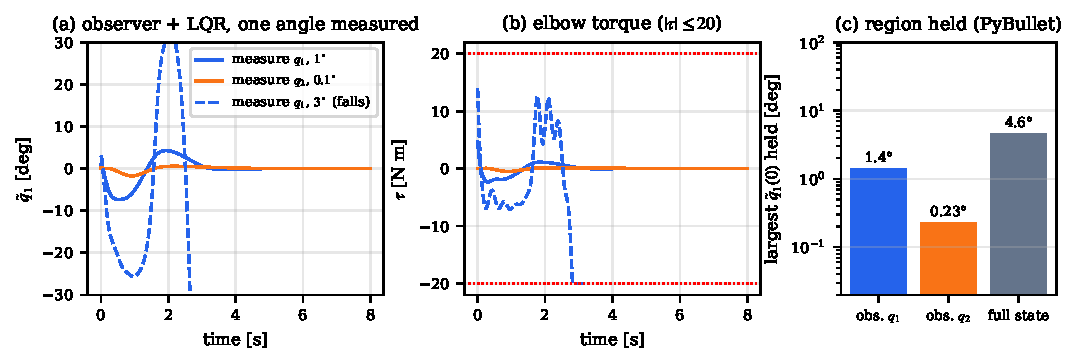
\includegraphics[width=0.92\textwidth]{fig_observer.pdf}
\caption{Observer + LQR at $E_3$ in PyBullet using one measured angle. (a) $\tilde q_1$; (b) elbow torque; (c) largest initial offset $\tilde q_1(0)$ that is still stabilized.}\label{fig:obs}
\end{figure}

\subsection{Answer}
\textbf{No static or PD feedback from a single joint angle can stabilize the upright equilibrium}, for either $q_1$ or $q_2$. Each $G_j$ at $E_3$ has a real zero in the RHP, and that forces the sign conflict in~\eqref{eq:pdpoly}: high gain drags a pole onto the RHP zero, and low gain leaves the RHP poles in place. Stabilization from one angle \textbf{is} possible with a \emph{dynamic} controller, because each angle alone makes the system observable. But the RHP zero sits next to the RHP pole $2.24$, which makes any such loop extremely fragile. With $|\tau|\le20\Nm$ it holds only $\approx1.4^\circ$ (via $q_1$) or $\approx0.2^\circ$ (via $q_2$, where the controller must even be unstable). Full-state feedback is the practical route for Phase~3.

% =====================================================================
\section{Simulation Tools}
% =====================================================================
\begin{itemize}
\item \textbf{Interactive PyBullet simulator}: \texttt{phase2/acrobot\_phase2\_sim.py}. Instructions are in \texttt{phase2/README.md}. A live dashboard lets you pick an equilibrium, an initial condition (slider, typed value, or by dragging the arm), and a controller: open loop, single-angle PD, or single-angle observer + LQR. It shows the nonlinear arm next to the linear model, $\tilde q(t)$, $\tau(t)$ and the closed-loop poles in the $s$-plane, all updating live.
\item \textbf{Reproducibility}: every figure and number above is produced by \nolinkurl{phase 2 deliverable/code/make_phase2_results.py}, run on the same simulator.
\item \textbf{Phase~2 animation} (Manim, 2K): \href{https://drive.google.com/file/d/19THfoXXzbdMtbteCKE4v0VRLpV869wE0/view?usp=sharing}{\textcolor{blue!60!black}{\textbf{watch the video}}}.
\end{itemize}

\vspace{6pt}
\begin{singlespace}
{\footnotesize
\textbf{References.}
[1] M.~W. Spong, ``The swing up control problem for the Acrobot,'' \emph{IEEE Control Syst. Mag.}, vol.~15, no.~1, pp.~49--55, 1995.\quad
[2] R.~Tedrake, \emph{Underactuated Robotics}, MIT, 2024. [Online]. Available: https://underactuated.csail.mit.edu\quad
[3] S.~Skogestad and I.~Postlethwaite, \emph{Multivariable Feedback Control}, 2nd ed., Wiley, 2005.\quad
[4] D.~C. Youla, J.~J. Bongiorno and C.~N. Lu, ``Single-loop feedback-stabilization of linear multivariable dynamical plants,'' \emph{Automatica}, vol.~10, pp.~159--173, 1974.\quad
[5] H.~K. Khalil, \emph{Nonlinear Systems}, 3rd ed., Prentice Hall, 2002.\quad
[6] E.~Coumans and Y.~Bai, ``PyBullet, a Python module for physics simulation,'' 2016--2024. [Online]. Available: https://pybullet.org\par}
\end{singlespace}

\end{document}
